\documentclass[dvipdfmx,11pt]{beamer}

% 数式
\usepackage{amsmath,amssymb,bm} %数式環境
\usepackage{mathtools}
\usepackage{physics}
\usepackage{autobreak}

% 画像
\usepackage{graphicx}
\usepackage[dvipdfmx]{color}

% 脚注
\usepackage[hang,small,bf]{caption}

% 括弧
\newcommand{\Bigparen}[1]{\Bigl(#1\Bigr)}
\newcommand{\Bigbrace}[1]{\Bigl\{#1\Bigr\}}
\newcommand{\Bigbrac}[1]{\Bigl[#1\Bigr]}
\newcommand{\Biggparen}[1]{\Biggl(#1\Biggr)}
\newcommand{\Biggbrace}[1]{\Biggl\{#1\Biggr\}}
\newcommand{\Biggbrac}[1]{\Biggl[#1\Biggr]}

\usefonttheme{professionalfonts} %数式フォントをいつも通りにする
\usetheme{metropolis} % Use metropolis theme



\title{}
\author{}
\date{\today}
\institute{所属機関}
\begin{document}
\maketitle

\begin{frame}{目次}
  \tableofcontents
\end{frame}


\section{セクション1}

\begin{frame}
  \frametitle{Introduction: The community detection from the perspective of physics}

  Approach to the community detection problem
  \begin{itemize}
    \item Min Bisection
    \begin{itemize}
      \item Optimizing the objective function (e.g. modularity) for a given network
      \item Maximizing is NP-hard but it performs well in real-world networks
      \item However, model sometimes overfits to the data 
    \end{itemize}

  \end{itemize}

    \begin{columns}
      \begin{column}{0.4\textwidth}
        \begin{figure}
          \centering
          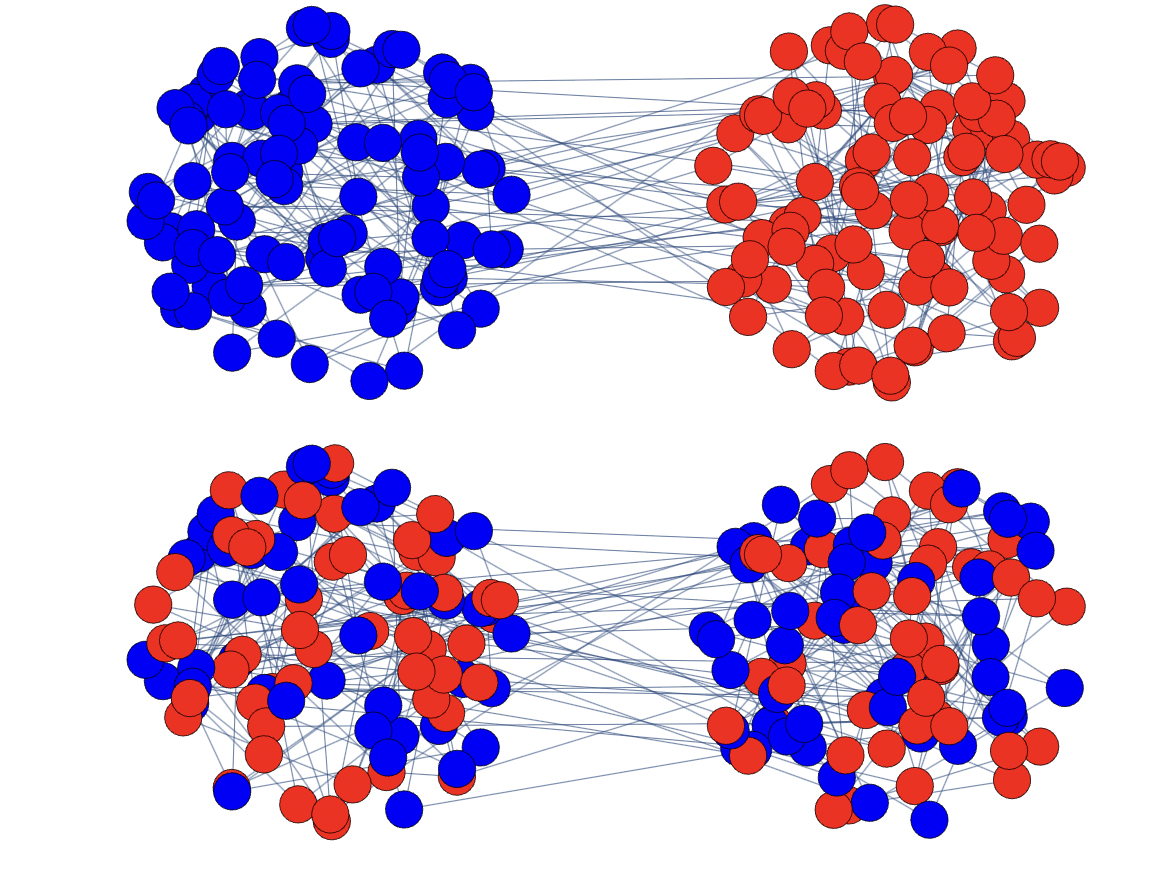
\includegraphics[width=0.8\linewidth]{figure/overfit.png}
          \caption{Partition of a random graph}
        \end{figure}
      \end{column}
  
      \begin{column}{0.60\textwidth}
        \begin{itemize}
          \item The top partition has 38 edges crossing while the bottom one has 39.
          \item For optimzer, the top one is ''optimal" but actually there is no community. 
        \end{itemize}
      \end{column}
    \end{columns}
\end{frame}



\begin{frame}
  \frametitle{Introduction: The community detection from the perspective of physics}

  \begin{itemize}
      \item In computer science, we think \alert{worst-case instances} for evaluating algorithms.
      \item However, the real world networks are rarely worst-case instances.
      \item In physics, we think \alert{typical instances} for evaluating models. (e.g. thermodynamics) \\
      $\Rightarrow$ It is natural to use physical perspective to evaluate the community detection models.
  \end{itemize}
\end{frame}



\begin{frame}
  \frametitle{二段組}

  \begin{columns}
    \begin{column}{0.48\textwidth}
        \begin{itemize}
          \item 文字
          \item 表
        \end{itemize}
    \end{column}

    \begin{column}{0.48\textwidth}
        \begin{figure}
          \centering
          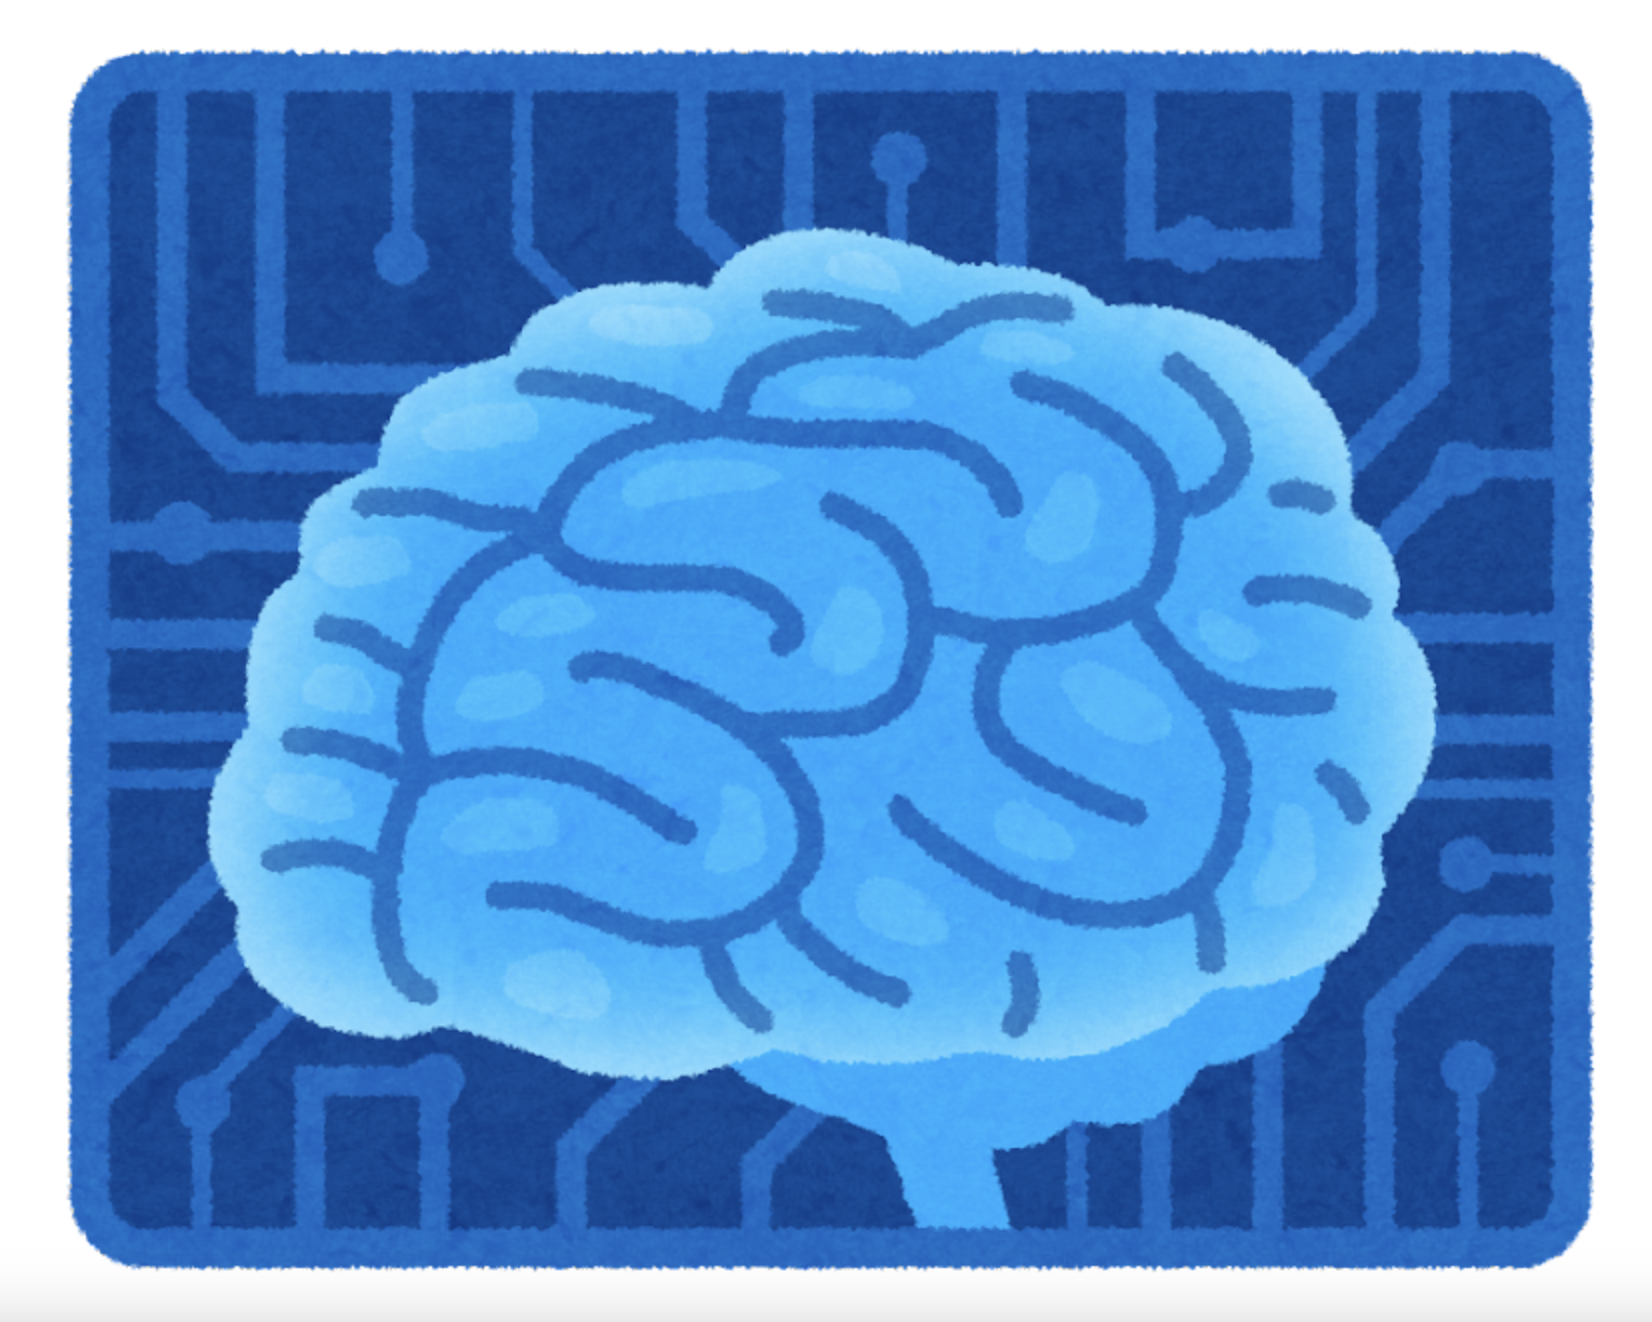
\includegraphics[width=0.8\linewidth]{figure/sample.png}
          \caption{図}
        \end{figure}
    \end{column}
  \end{columns}


\end{frame}


\begin{frame}
  \frametitle{Problem setting}
  \begin{itemize}
    \item Sparse and symmetric stochastic block model (SBM)
    \begin{itemize}
      \item $n$:  $\#$ nodes
      \item $q$:  $\#$ communities
      \item each node $i$ belongs to a community $\sigma_i \in \{1, \dots, q\}$
      \item if $i$ and $j$ belong to the same community, $A_{ij} \sim \text{Bern}(p_{in})$
      \item 
    \end{itemize}
  \end{itemize}

  

\end{frame}





\end{document}




